\documentclass[tikz,dvisvgm]{standalone}
\usetikzlibrary{decorations.markings}
\usetikzlibrary{decorations.text}
\usetikzlibrary{shapes,arrows,calc}
\usetikzlibrary{patterns,patterns.meta} 

\def\PlotForces{}
\def\PlotRadius{}
% \def\PlotKinematics{}

\begin{document}
    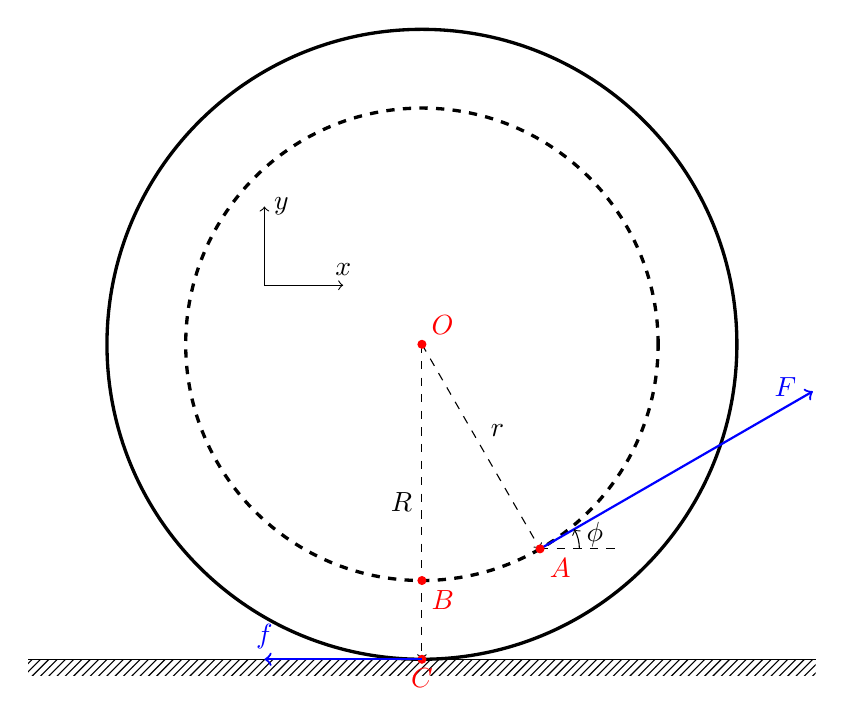
\begin{tikzpicture}
        \coordinate (O) at (0, 0);
        \coordinate (A) at (-60:3);
        \coordinate (B) at (0, -3);
        \coordinate (C) at (0, -4);
        \draw [very thick] (0, 0) circle (4);
        \draw [very thick, dashed] (0, 0) circle (3);
        \ifdefined\PlotKinematics
            \draw [blue, thick, ->] (0, 0) -- (3, 0) node [above right] {$\vec v_O$};
            \draw [dashed] (0, 0) -- (0, -4);
        \fi
        
        \begin{scope}[rotate=-60]
            \begin{scope}[xshift=3cm]
                \begin{scope}[rotate=60]
                    \ifdefined\PlotForces
                        \draw [blue, thick, ->] (0, 0) -- (30:4) node[pos=0.9, above] {$F$};
                        \draw [dashed] (0, 0) -- (1, 0);
                    \draw [->] (0.5, 0) arc (0:30:0.5) node [pos=0.7, right] {$\phi$};
                    \fi
                    \ifdefined\PlotKinematics
                        \coordinate (vaend) at ($(A)!1.54cm!90:(C)$);
                        \draw [blue, thick, ->] (0, 0) -- (vaend) node [right] {$\vec v_A$};
                    \fi
                \end{scope}

                \ifdefined\PlotKinematics
                    \draw [dashed] (-1.5, 0) -- (1, 0);
                    \draw [dashed] (0, 0) node (newaxiso) {} -- (0, 1) node (newaxisy) {};
                    \coordinate (vatend) at ($(newaxiso)!(vaend)!(newaxisy)$);
                    \draw [blue, thick, ->] (0, 0) -- (vatend) node [right] {$\vec v_{A}^{\mathrm{t}}$};
                    \draw [blue, dashed] (vaend) -- (vatend);
                \fi
            \end{scope}
        \end{scope}
        \ifdefined\PlotKinematics
            \draw [dashed] (0, -4) -- (-60:3);
            \draw [blue, thick, ->] (0, -3) -- (0.75, -3) node[above] {$\vec v_B$};
            \begin{scope}[rotate=-20, xshift=3cm]
                \coordinate (Aprime) at (0, 0);
                \coordinate (vaprimeend) at ($(Aprime)!1.9cm!-90:(C)$);
                \filldraw [red] (Aprime) circle (0.05) node [above right] {$A'$};
                \draw [dotted] (C) -- (Aprime);
                \draw [dotted] (O) -- (Aprime) -- (0, 1);
                \draw [dotted] (Aprime) -- (1, 0);
                \draw [blue, thick, densely dotted, ->] (Aprime) -- (vaprimeend) node [above] {$\vec v_{A'}$};
                \draw [blue, thick, densely dotted, ->] (Aprime) -- ($(Aprime)!(vaprimeend)!(0, 1)$) node [right] {$\vec v_{A'}^{\mathrm{t}}$};
                \draw [blue, dotted] (vaprimeend) -- ($(Aprime)!(vaprimeend)!(0, 1)$);
            \end{scope}
        \fi

        \ifdefined\PlotRadius
            \draw [dashed, ->] (0, 0) -- (0, -4) node [pos=0.5, left] {$R$};
            \draw [dashed, ->] (0, 0) -- (-60:3) node [pos=0.5, above right] {$r$};
        \fi
        
        \draw (-5, -4) -- (5, -4);
        \fill [pattern={north east lines}] (-5, -4) rectangle +(10, -0.2);

        \filldraw [red] (O) circle (0.05) node[above right] {$O$};
        \filldraw [red] (C) circle (0.05) node[below] {$C$};
        \filldraw [red] (B) circle (0.05) node [below right] {$B$};
        \filldraw [red] (A) circle (0.05) node [below right] {$A$};
        \ifdefined\PlotForces
            \draw [blue, thick, ->] (0, -4) -- (-2, -4) node [above] {$f$};
        \fi

        \begin{scope}[xshift=-2cm, yshift=0.75cm]
            \draw [->] (0, 0) -- (1, 0) node [above] {$x$};
            \draw [->] (0, 0) -- (0, 1) node [right] {$y$};
        \end{scope}
    \end{tikzpicture}
\end{document}
